\chapter{Introduzione al progetto}
Per andare in banca si puo prendere la macchina, l’autobus, il  pc ed oggi il cellulare facendo tutte quelle operazioni che normalmente si fanno nelle filiali con il vantaggio di gestire i rapporti con la banca ovunque ci si trovi, 24 ore su 24, in meno tempo.
 
Infatti negli ultimi anni  si è manifestato un radicale cambiamento nel mondo finanziario che ha portato gli operatori del settore, in primo luogo le banche, non solo ad adeguare i propri servizi finanziari alla nuova realtà digitale ma anche a sviluppare nuove soluzioni capaci di indurre il cliente a gestire in modo nuovo il proprio denaro, fornendo servizi personalizzati alle diverse esigenze e alle abitudini di ogni singolo utente.
Le banche quindi hanno cominciato un processo di snellimento delle procedure e di semplificazione delle relazioni con la clientela grazie al quale si è parlato di \emph{banca a distanza} per indicare questo nuovo modus operandi che non richiede più la necessità di recarsi presso gli sportelli bancari.
Oggi la clientela può eseguire molte operazioni di sportello dalla propria casa, dal proprio ufficio, da un luogo qualsiasi in un momento qualsiasi della giornata utilizzando tecnologie più o meno avanzate.

Il mobile banking permette di fare banca a distanza ed ha una platea di utenza molto ampia data la diffusione degli smartophone e tablet che sta cambiando le modalità di offrire servizi e fare comunicazione o marketing da parte delle aziende comprese le banche che sperano nel giro di pochi anni di raggiungere quasi tutti i possessori di conto corrente. I servizi di mobile banking si propongono di raggiungere anche quegli utenti che non utilizzano l’home banking come i giovani, i disabili che nel mobile banking  non trovano barriere, gli immigrati che possono avere con questo canale un contatto più semplice e rapido con la banca e, non ultimi, gli anziani che sono meno avezzi all’uso delle tecnologie e non sanno bene districarsi tra password e tecnicismi.
Il mobile banking si rivela utile in tempi di crisi economica come quelli attuali, crisi che spinge i consumatori a usare nuovi canali di distribuzione dei servizi per risparmiare tempo e denaro. Infatti da indagini di mercato emerge che gli utenti del mobile banking sentono di avere più controllo del proprio denaro.
Le banche che forniscono questo servizio utilizzano strumenti in grado di rendere il cliente autonomo nella gestione dei proprio risparmi. Statistiche del settore dichiarano che la maggior parte degli utenti dichiara di andare meno in rosso e una buona percentuale di essi affermano di risparmiare di più utilizzando il mobile banking. Questo fenomeno è dovuto probabilmente alla frequenza con cui i clienti accedono al proprio conto. 

Il mobile banking è principalmente scelto perchè permette di avere la banca sempre vicino a se e di conseguenza  di risparmiare tempo. I clienti per il futuro si aspettano nuovi si sistemi di interazione con la banca come ad esempio sistemi di alert che l’informino che il conto è in rosso o consigli e informazioni su come gestire i propri investimenti e risparmi.
Oltre a consentire di effettuare le classiche operazioni bancarie in maniera diversa, il mobile banking cambia anche l’approccio dei  risparmiatori, i suoi comportamenti e perfino le sue decisioni finanziarie portando il risparmiatore ad avere più potere.

\section{Descrizione dell'applicazione}

L'applicazione permetterà a qualsiasi cliente dell'istuto bancario di poter usufruire della maggior parte dei servizi messi a disposizione dello stesso. In particolare l'applicazione permetterà all'utente di poter ricevere sempre informazioni dettagliate e aggiornate sullo stato dei suoi conti e delle sue carte, dei movimenti effettuati e di poter eseguire in ogni momento diverse operazioni bancarie ovunque esso si trovi in totale mobilità. Oltre i classici servizi, l'applicazione permetterà all'utente di poter navigare tra i contenuti social e le offerte dedicate ai correntisti messi a disposizione dai canali diretti della banca e di condividere tali informazioni sui social network.
L'applicazione offrirà inoltre la possibilità all'utente di contattare direttamente l'istituto bancario e di poter prenotare appuntamenti con consulenti specializzati e permetterà di ricevere messaggi ed e-mail sullo stato del conto, sui movimenti effettuati e messaggi di carattere informativo, inviati direttamente dalla banca.


\section{Primi requisiti funzionali}
Di seguito sono riportati i primi requisiti funzionali ricavati dal processo di analisi delle richieste del committente, ottenute durante le interviste iniziali del progetto. Tali requisiti definiscono le funzionalità e i servizi 
offerti dal sistema da realizzare.

\begin{center}
       \captionof{table}{Primi requisiti funzionali}

    \begin{tabular}{p{6cm}|p{8cm}}

    \toprule
    \multicolumn{1}{c}{\textbf{Requisito funzionale}} &
    \textbf{Descrizione}\\

    \midrule
    Login ai servizi & Permettere all'utente l'accesso ai servizi bancari mediante credenziali \\\\
    Visualizzazione riepilogo conti e carte & Fornire opportune viste di riepilogo dei prodotti posseduti da un utente (esempio: conti correnti, carte di credito, ecc\dots)\\\\
    Visualizzazione storico saldi & Rappresentare tramite grafici dello storico saldi di un prodotto\\\\
    Riepilogo lista movimenti & Recuperare e visualizzare la lista dei movimenti di un determinato prodotto\\\\
    Filtraggio lista movimenti & Permettere il recupero dei movimenti in base un certo arco temporale\\\\
    Disporre operazioni bancarie & Permettere l'esecuzione di dispositive bancarie (esempio: bonifici, giroconti, ecc\dots) \\\\
    Interazione con i social network & Consentire la visualizzazione dei contenuti social messi a disposizione del cliente\\\\
    Messaggistica & Permettere la lettura delle comunicazioni ricevute  \\\\
    \bottomrule

    \end{tabular}
        \label{tab:requisiti_iniziali}

\end{center}



\section{Primi mockup, wireframe e prototipi}
\subsection{Mockup}
La realizzazione di mockup grafici ha permesso di offrire al cliente una prima rappresentazione visiva dei requisiti funzionali iniziali. Di seguito sono riportate alcuni di questi mockup relativi allo stadio iniziale del progetto.

\begin{figure}[!htbp]
\centering
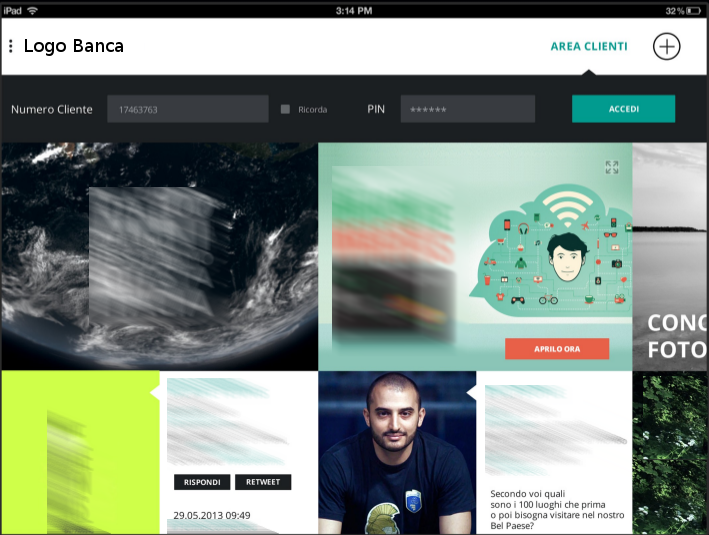
\includegraphics[scale=0.7]{immagini_mockup/home.png}
\caption{Home contenuti social e pannello login}
\end{figure}

\begin{figure}[!htbp]
\centering
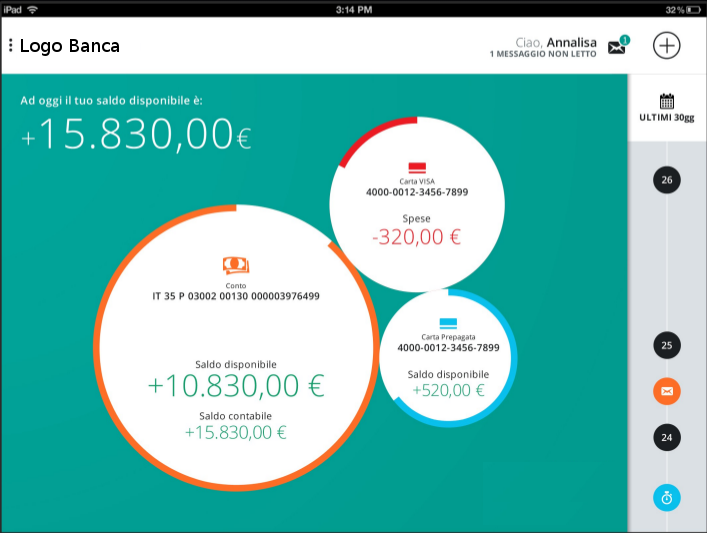
\includegraphics[scale=0.7]{immagini_mockup/bolle.png}
\caption{Riepilogo conti e carte}
\end{figure}

\begin{figure}[!htbp]
\centering
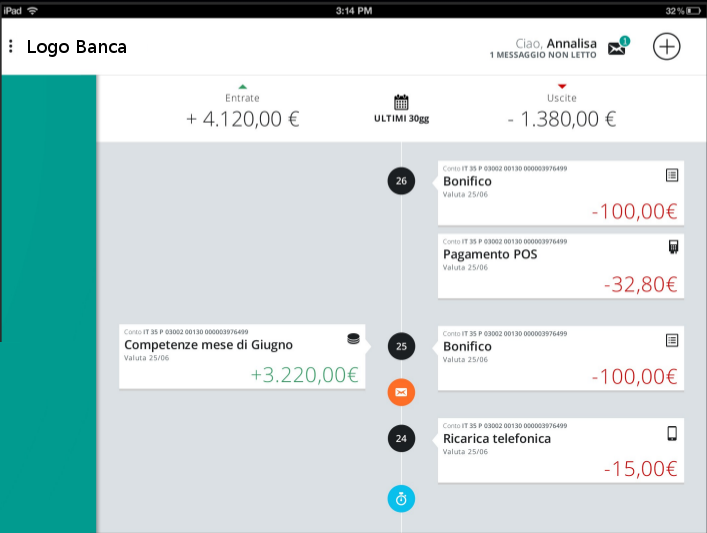
\includegraphics[scale=0.7]{immagini_mockup/timeline.png}
\caption{Timeline movimenti}
\end{figure}

\begin{figure}[!h]
\centering
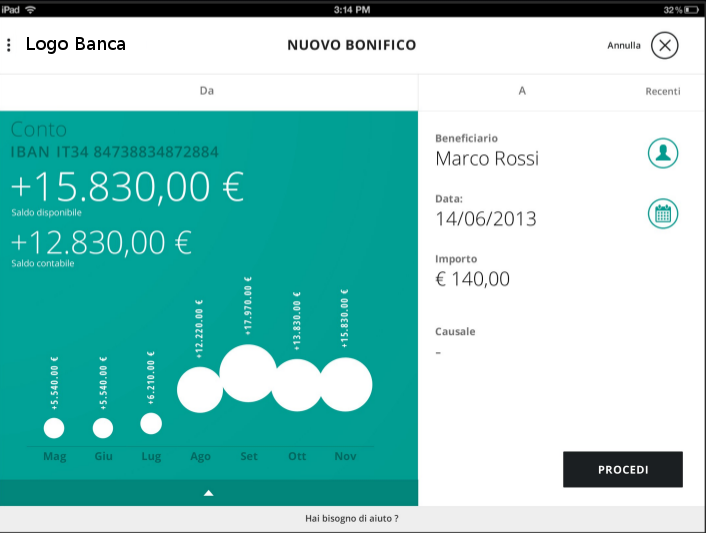
\includegraphics[scale=0.7]{immagini_mockup/bonifico.png}
\caption{Operazione bonifico}
\end{figure}

\newpage
\subsection{Wireframe}
Parallelamente ai mockup e durante tutto il ciclo di vita del software sono stati realizzati e raffinati i wireframe. 

I wareframe forniscono una rappresentazione strutturale di un applicazione software e permettono di individuare le dinamiche del progetto in termini di usabilità ed utilizzo pratico, i punti critici e quelli che richiedono uno sviluppo più accurato o miglioramenti.

Di seguito sono mostrate alcune delle immagini di uno dei primi wireframe realizzati:

\begin{figure}[!htbp]
\centering
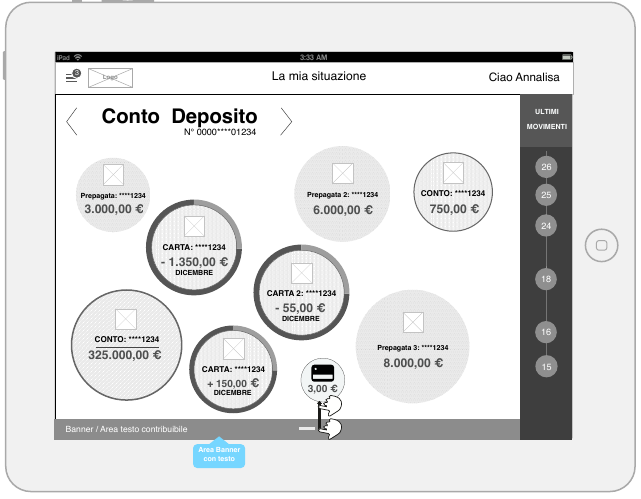
\includegraphics[scale=0.85]{primo_wireframe/miasituazione.png}
\caption{Riepilogo conti e carte}
\end{figure}
\begin{figure}[!htpb]
\centering
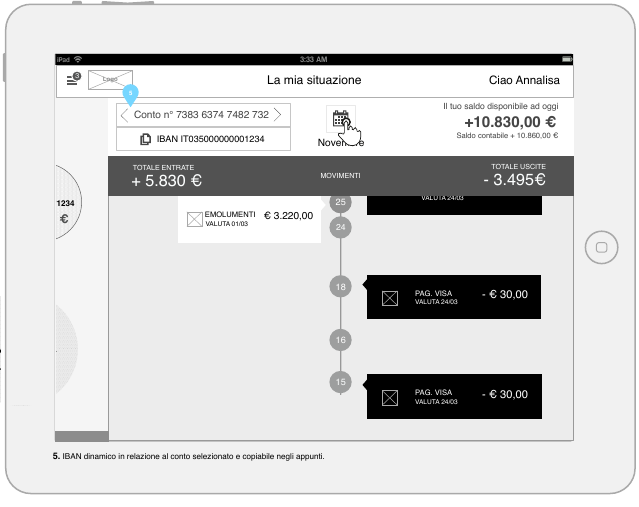
\includegraphics[scale=0.85]{primo_wireframe/timeline2.png}
\caption{Timeline movimenti}
\end{figure}
\begin{figure}[!htbp]
\centering
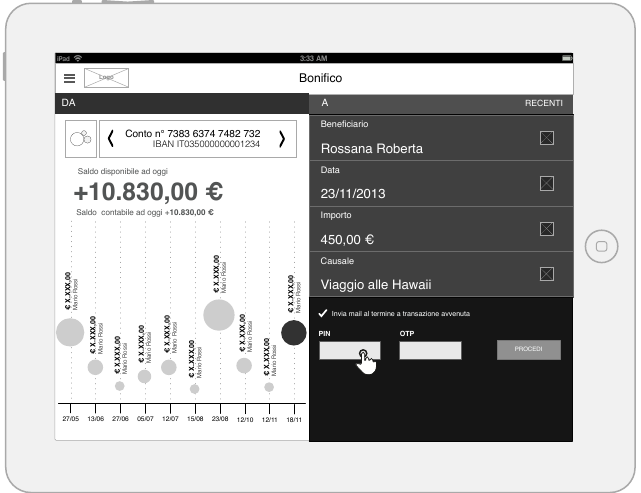
\includegraphics[scale=0.85]{primo_wireframe/bonifico2.png}
\caption{Dettaglio bonifico}
\end{figure}

\newpage
\subsection{Prototipi}
Un'altro passo fondamentale durante la fase iniziale del progetto è stato la realizzazione di prototipi.

Un prototipo è un modello approssimato del sistema che si sta realizzando e che simula o esegue solo una parte delle funzioni del sistema finale.
La prototipizzazione permette di:

\begin{itemize}
  \item tenere il design centrato sull’utente 
  \item sperimentare design alternativi
  \item ottenere feedback rapidi sul progetto
  \item trascurare dettagli secondari (come qualità del codice, efficienza, ecc\dots) 
  \item valutare l'usabilità
  \item ridurre i rischi di un progetto permettendoci di mettere prima a fuoco alcune caratteristiche del sistema e capire se sono adeguate o meno
\end{itemize}

Durante le prime settimane del progetto sono stati quindi realizzati dei prototipi contenenti funzionalità \emph{stub}\footnote{Funzionalità che simulano il comportamento  del sistema restituendo valori accettabili in un ipotetico scenario reale.} descritte dalla tabella \ref{tab:requisiti_iniziali}. Tali prototipi sono stati successivamente messi a disposizione del cliente e testati su device Apple iPad, portando alla raccolta e valutazione dei primi feedback sull'utilizzo del software.
